\section{Empirical Evaluation}
\label{sec:evaluation}

\todo{Fill it up with juicy bits once we actually have them graphs.}

\subsection{Experimental Setup}

\paragraph{Algorithms}

We implemented the low rank recovery optimization routines for $M_2$ and
$M_3$ using a proximal subgradient descent algorithm\citationneeded. The
algorithm was initialized with the regularized least squares solution
and was run to convergence in each instance. Both regularization
parameters were annealed as $\frac{1}{T}$. 

As a baseline, we also implemented EM with two different
initializations. For the first, we used $\beta$s with random standard
Gaussian entries and uniform mixture probabilities, $\pi$. In the other,
we initialized EM with the starting points given by Spectral Experts. 

\paragraph{Datasets}

We generated synthetic data using covariates from the unit hyper cube
and non-linear responses.  To conform to the identifiability criteria
discussed in \sectionref{sec:algo}, we considered only features that
would guarantee this condition. 

As an example, one set of features we considered in the uni-dimensional
setting were $\{1, x, x^4, x^7\}$. The data and the curves fit using
Spectral Experts, EM with random initializations and EM initialized with
the parameters recovered using spectral experts are shown in
\figureref{fig:curves}.

\begin{figure*}[t]
  \centering
  \subfigure[Spectral]{
    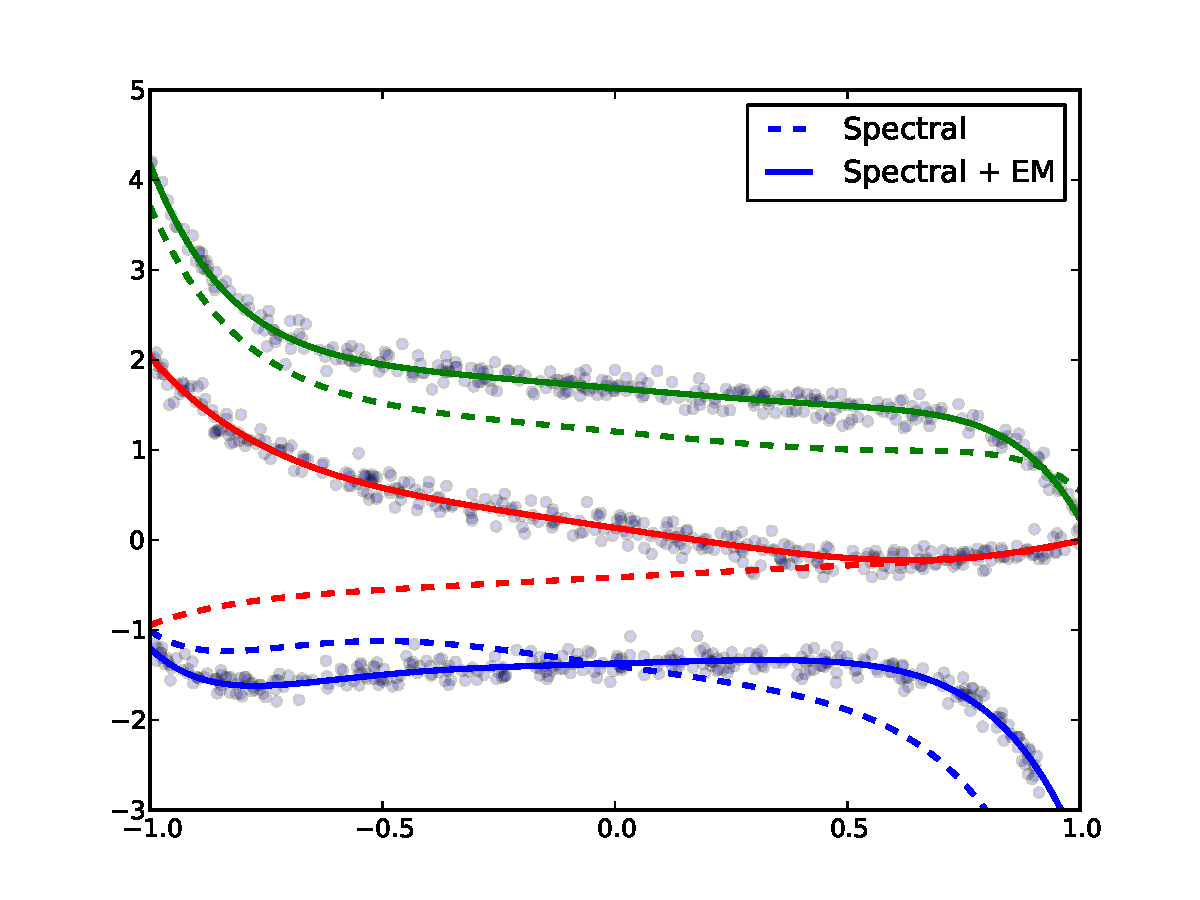
\includegraphics[width=0.50\textwidth]{figures/curves-vis/1-8-3-specm.pdf}}
    \hspace{-2em}
  \subfigure[EM]{
    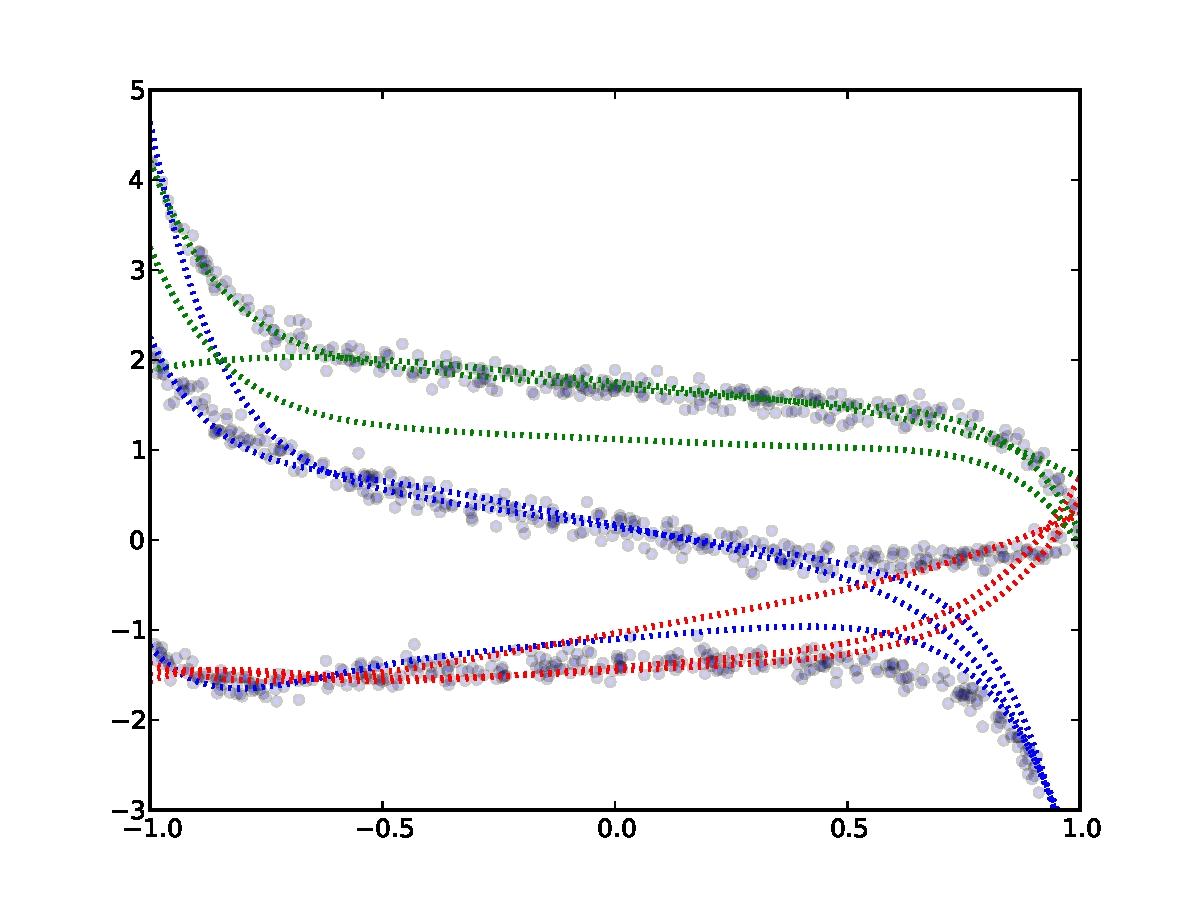
\includegraphics[width=0.50\textwidth]{figures/curves-vis/1-8-3-em.pdf}}
    \hspace{-2em}
%  \subfigure[Spectral + EM]{
%    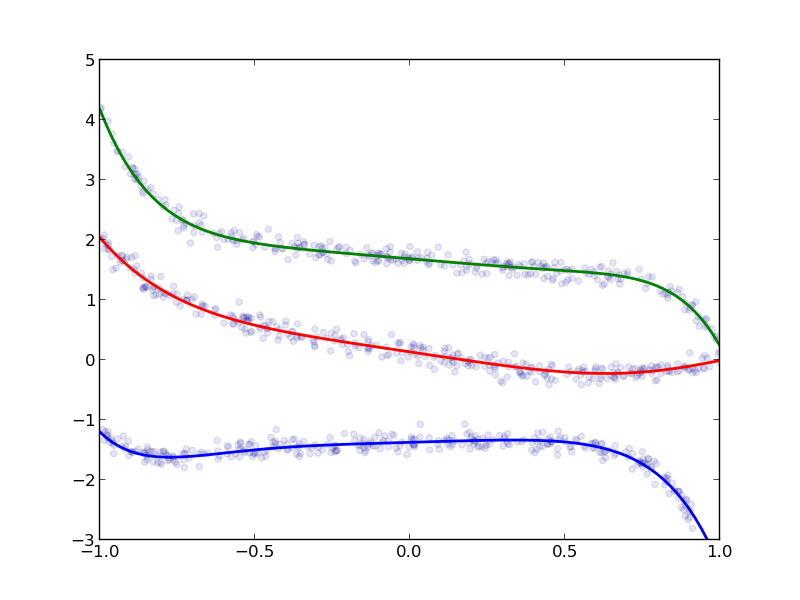
\includegraphics[width=0.34\textwidth]{figures/curves-vis/1-8-3-spem.png}}
  \caption{A comparison between SpectralExperts and EM. The dashed lines
  on the left denote the solution recovered by Spectral Experts. Whilst
  not a perfect fit, it provides an good initialization for EM to find
  the true global minima. The dotted lines on the right show different
  local optima found by EM on this example.}
  \label{fig:curves}
\end{figure*}

%Default values:
%$n = 10^6$
%$k = 5$

\begin{table*}[t]
\caption{Parameter Recovery ($N = 500,000$).}
\label{tbl:parameter-recovery}
\vskip 0.15in
\begin{center}
\begin{small}
\begin{sc}

  \begin{tabular}{ >{\centering}p{5cm}<{\centering} r c c c }
\hline
\abovespace\belowspace
Features  & $K$ & Spectral & EM & Spectral + EM \\
\hline
\abovespace
$\{1$, $ x_1$, $ x_1^4\}$ 
  & 2 & 2.54 $\pm$ 2.81 & 0.28 $\pm$ 0.82 & 0.13 $\pm$ 0.55 \\
$\{1$, $ x_1$, $ x_2$, $ x_1^2 x_2^2\}$ 
  & 3 & 3.93 $\pm$ 5.82 & 0.33 $\pm$ 0.96 & 0.35 $\pm$ 1.23 \\
$\{1$, $ x_1$, $ x_2$, $ x_1 x_2^3$, $ x_1^2 x_2^2$, $ x_1^3 x_2 \}$ 
  & 5 & 5.27 $\pm$ 2.32 & 1.80 $\pm$ 1.80 & 1.51 $\pm$ 1.77 \\
$\{1$, $ x_1$, $ x_2$, $ x_1 x_2^3$, $ x_1^2 x_2^2$, $ x_1^3 x_2$, $ x_1^3 x_2^4$, $ x_1^4 x_2^3 \}$ 
  & 7 & 8.42 $\pm$ 1.66 & 7.41 $\pm$ 2.99 & 7.31 $\pm$ 2.47 \\
$\{1$, $ x_1$, $ x_2$, $ x_3$, $ x_1 x_2 x_3^2$, $ x_1 x_2^2 x_3$, $ x_1^2 x_2 x_3$, $ x_1^2 x_2^2$, $ x_1^2 x_3^2$, $ x_2^2 x_3^2$, $ x_3^2\}$
  & 3 & 3.78 $\pm$ 0.90 & 0.67 $\pm$ 1.49 & 0.51 $\pm$ 1.12 \\
$\{1$, $ x_1$, $ x_2$, $ x_3$, $ x_1 x_2 x_3^2$, $ x_1 x_2^2 x_3$, $ x_1^2 x_2 x_3$, $ x_1^2 x_2^2$, $ x_1^2 x_3^2$, $ x_2^2 x_3^2$, $ x_3^2\}$
  & 7 & 9.97 $\pm$ 3.22 & 1.43 $\pm$ 1.97 & 1.42 $\pm$ 2.17 \\
\hline
\end{tabular}
\end{sc}
\end{small}
\end{center}
\vskip -0.1in
\end{table*}

\todo{Dataset 2}: $b = 30$, $p = 1$ [TODO]



\paragraph{Motion tracking data?}

\subsection{Results}

\paragraph{Basic results}

Punchline: spectral by itself is medicore, offers a good initialization to EM.
EM with random initialization is much less stable. (by table)

Using canonical settings, on the various datasets

Plot the parameters: the curves, three algorithms (DONE)

Plot: the histogram over errors (for EM?)

\paragraph{Misspecified Data}

To show how well spectral methods can handle mis-specification, we
compared the performance of the different algorithms with entire
segments removed from the generated data. \todo{Table X shows figures}.

\paragraph{Effect on number of data points}

\begin{figure}[t]
  \centering
  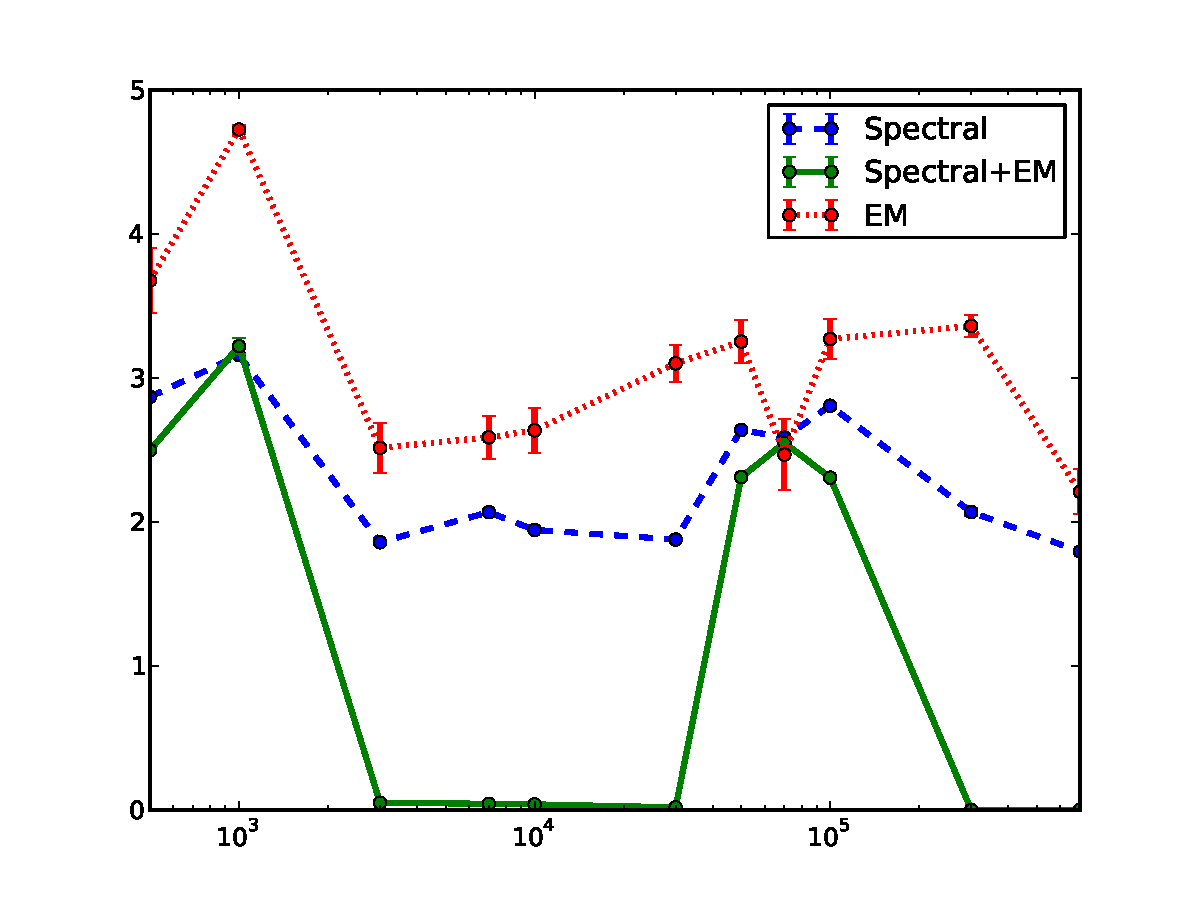
\includegraphics[width=0.45\textwidth]{figures/vs-n/1-8-3-3.pdf}
  \caption{}
  \label{fig:vs-n}
\end{figure}

\todo{We see that the error of spectral is actually less than EM after a point.}

Point: tradeoff between statistical error and computational error;
not enough data, spectral is actually a lot worse
given enough data, spectral+EM is much better

\paragraph{Effect of noise}

\paragraph{Effect of separation between components}
